\chapter{Results}\label{ch:results}

\section{The experiences dataset}\label{sec:resdataset}
In total, 38 scientists were invited to interview and, of the 20 who responded, 14 participants were available and interviewed during the period of this study (July and August 2024). A broad categorisation of participants' background science and their current focus (science or policy) is given in Table~\ref{tab:cohort}. Participants represented, broadly, biophysical sciences, social scientists or were cross-disciplinary. Whilst the biophysical scientists were mostly involved in measurement, monitoring and modelling of the biological and physical environment, three participants had had some involvement in research related to negative emissions, and related, technologies. Participants' current roles also spanned from being primarily focused on scientific research to being focused on supporting policy with scientific knowledge, with four participants being based in non-academic, government-related organisations (whilst also maintaining links to academia). In total there was 9\textonehalf{} hours of interviews, transcribed into 1441 statements. The majority of statements received one or more indicator label.

% \begin{table}
% \centering
% \footnotesize
% \caption{Caption}\label{tab:cohort}
% \begin{tabular}{L{.18\linewidth}L{.08\linewidth}L{.08\linewidth}}
% \textbf{current focus} & \textbf{female} & \textbf{male} \\ \hline
% \multicolumn{3}{c}{\small \textbf{biophysical}}\rule{0pt}{4ex} \\
% science & 3 & 1 \\ 
% policy	& 1 & 3 \\[2mm] \hline
% \multicolumn{3}{c}{\small \textbf{social science}}\rule{0pt}{4ex} \\
% science	& 1 &	1 \\ 
% policy	& 2 &	\\[2mm] \hline
% \multicolumn{3}{c}{\small \textbf{cross-disciplinary}}\rule{0pt}{4ex} \\ 
% science & & 1 \\ 
% policy	 & & 1 \\[2mm] \hline
% \end{tabular}
% \label{tab:my_label}
% \end{table}

\begin{table}[!ht]
\centering
\footnotesize
\caption{Summary of this study's cohort, showing the count of female and male participants against their scientific background and current focus}\label{tab:cohort}
\begin{tabular}{B{.25\linewidth}L{.2\linewidth}L{.15\linewidth}L{.15\linewidth}} \hline
\textbf{background} & \textbf{current focus} & \textbf{female} & \textbf{male} \\ \hline \hline
\multirow{2}{*}{biophysical science} &
science & 3 & 1 \\ 
& policy	& 1 & 3 \\[2mm] \hline
\multirow{2}{*}{social science} &
science	& 1 &	1 \\ 
& policy	& 2 &	\\[2mm] \hline
\multirow{2}{*}{cross-disciplinary} & 
science & & 1 \\ 
& policy	 & & 1 \\[2mm] \hline
\end{tabular}
\label{tab:my_label}
\end{table}

With the data in \CSV{} format, a brief quantitative analysis was undertaken, using the R language, to determine if any strong quantitative patterns emerged from the data. This included determining the association between different \ISM{} factors and a manually assigned ``role'', and a cluster analysis over the indicator labels to determine if participants grouped into different ``types''. The results from this analysis were inconclusive and further quantitative analysis was not undertaken.

%A total of 155 stories\improvement{are stories relevant? if so explain in Chapter~\ref{ch:methods}} were identified in the interviews, excluding those pertaining to the participants' introductory statements about their field of work. Frequently, a story would contain multiple labels for the same theme. For instance, Story 45 ``frustrations as a scientist compared to those as a concerned citizen'' contained mentions of 3 different roles, as well as a description of a conflict in roles. Section~\ref{sec:resski} discusses the nature of each of the ISM factors as they surface within the interviews.

%\section{Influences and strategic activities}\label{sec:resski}
In the following, the factors of influence are differentiated using \textsc{Small Caps font}.

Having identified indicator labels for the factors in the \ISM{} framework, a number of factors were deemed rather ambiguous, whilst other factors had considerable overlaps. Further work resolved many of these conflicts by separating ``three systems'' from the narratives: \skiinte, \skiknow{} and \skiscip, as illustrated in Figure~\ref{fig:resski}. The most significant resolution was to combine the \ISM{} \ismsn, \ismst{} and some aspects of \ismsm{} into a new factor, \skipers, within the \skiinte. This new factor represented the \emph{perspective taking} that participants were performing about others, and to some extent the \emph{perspective taking} that participants inferred was taking place about scientists. 

\begin{figure}[!ht]
    \centering
    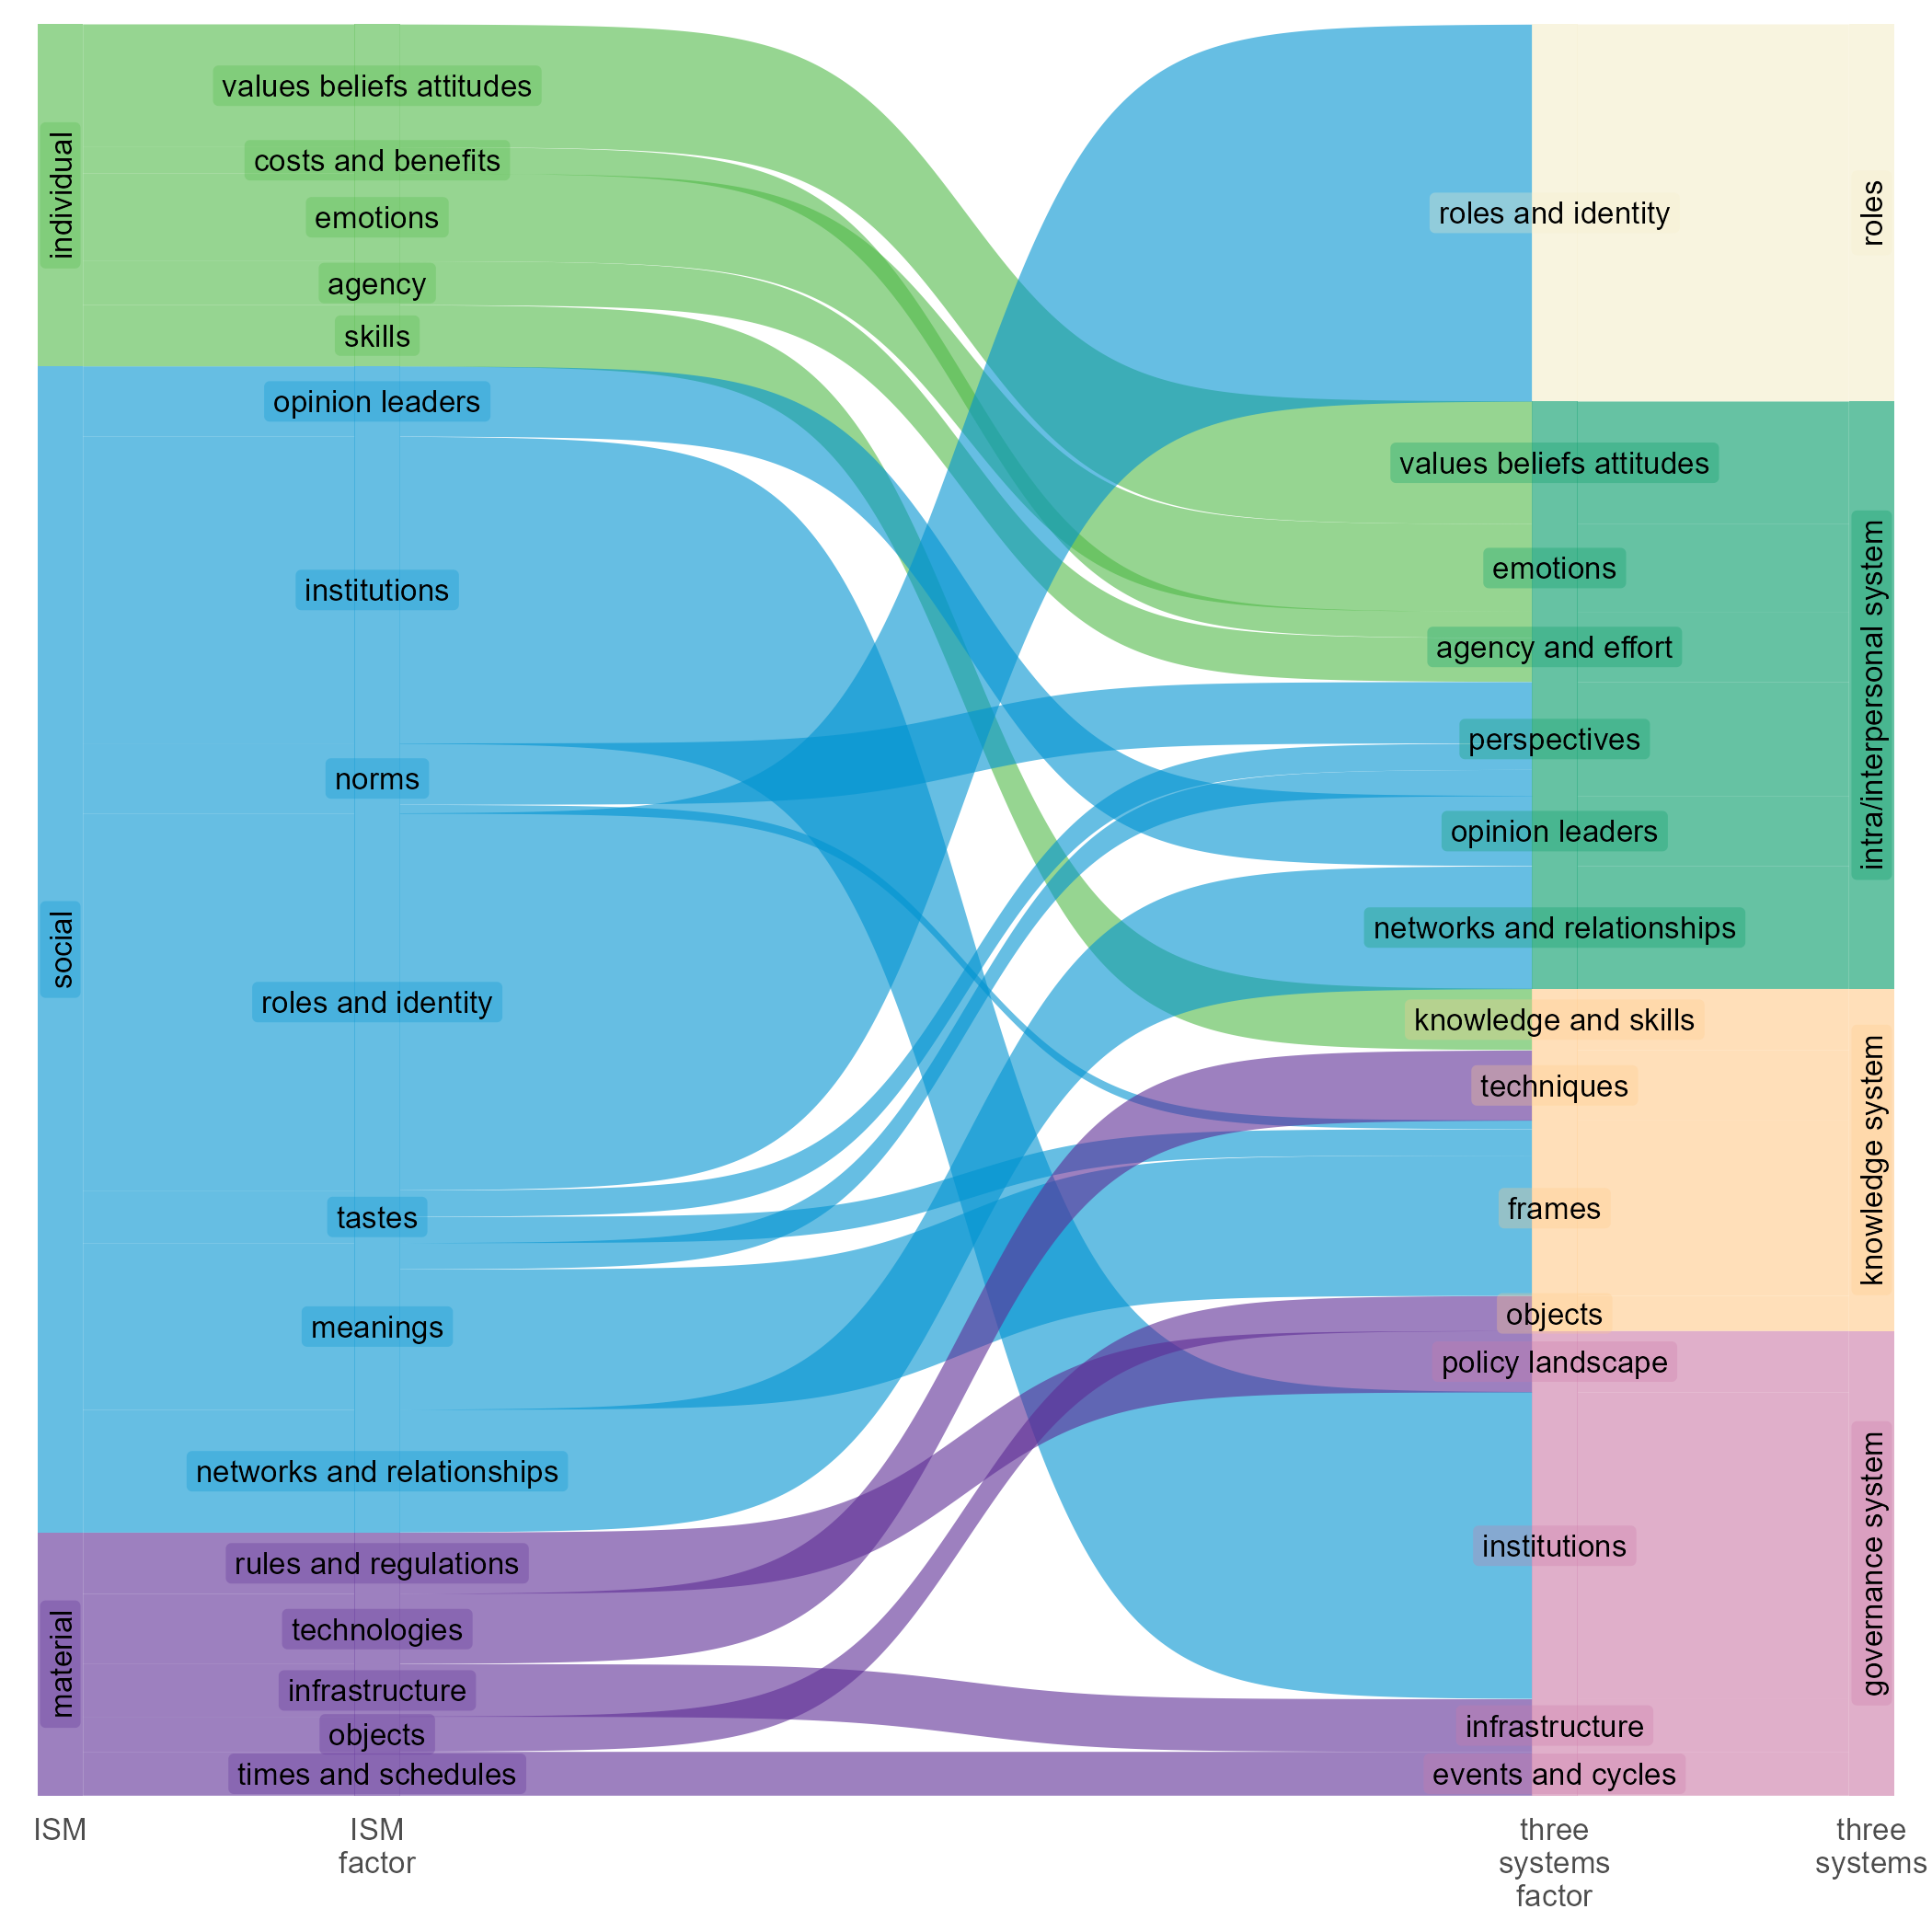
\includegraphics[width=1\linewidth]{figures/ISM_to_threesystems.png}
    \caption{Diagram showing how the \ISM{} factors were transposed into the three systems factors. The widths of the flows are proportional to the number of indicators for each factor.}
    \label{fig:resski}
\end{figure}

Having extracted \skipers{} indicators from \ismsm, the original \ISM{} factor comprised of indicators about issue and policy \emph{framings} and so was renamed \skifram, within the \skiknow. Another resolution was to combine \ISM{} \ismic{} and \ismia{} into \skiagen, within the \skiinte. Whilst the original two factors indicated subtly different influences, this was a pragmatic combination because the indicators often coexisted and \ismic{} was not a commonly featuring factor in the interviews. \ISM{} \ismmt{} was really as set of \skitech{} used to generate knowledge and was renamed thus, within the \skiknow. Similarly, \ISM{} \ismmr{} were observations about the \skipoli{} and \ismmts{} were observations about \skieven{}, both within the \skiscip.

The following sections outline the indicator labels and strategic practices that were identified for each factor. For each, the labels and practices are tabulated with illustrative quotes from the dataset. A measure of the influence of each indicator is provided in broad terms (\emph{enabling}, \emph{inhibiting}, \emph{neutral}, \emph{various}). The indicators and practices are further described within each section. Being a primary framework for theory about engagement with the \SPI, the results for \skirole{} were considered first, as described in Section~\ref{sec:resroles}. The results for the three interconnected systems are then described as follows: \skiinte: Section~\ref{sec:resskiinte}, \skiknow: Section~\ref{sec:resskiknow}, and \skiscip: Section~\ref{sec:resskiscip}. 

\section{Roles and identity}\label{sec:resroles}

\begin{table}[!ht]
\footnotesize
\caption{Indicators of \ismsr}\label{tab:resrole}
\begin{tabular}{L{.15\linewidth}L{.35\linewidth}L{.5\linewidth}} \hline
\textbf{id} & \textbf{indicator label} & \textbf{example quotes} \\ \hline \hline
roles & academic; adviser; advocate; broker; citizen; public servant; representative; researcher; specialist &  \tquote{if you wear an academic hat you can really speak your mind}{p04}{27} \vfill \tquote{I strongly prefer playing the broker, advisor role}{p09}{109} \\[2mm]\rule{0pt}{4ex}
\multirow{2}{.12\linewidth}{identities} & authoritative; candid; esteemed; experienced; expert; helpful; humble; impartial; informed; judicious; receptive; relevant; selfish & \tquote{that succeeded because of who I was and my reputation as an academic and an IPCC author}{p06}{85} (esteemed) \vfill \tquote{whereas as a ... civil servant, I was restricted in what I could say}{p04}{28} (judicious) \\[2mm] \rule{0pt}{4ex}
& undervalued & \tquote{... even just some ... acknowledgement or recognition that people are part of this ...}{p03}{64} \\ \hline
\end{tabular}
\end{table}


%Participants referred to theirs, or other scientists', roles or identity in about one fifth of the stories. 
Participants identified a varied set of roles for themselves and other scientists working at the \SPI{} (Table~\ref{tab:resrole}). As one participant noted, \tquote{scientists are a very diverse bunch}{p09}{60}. Participants with a science-focus saw their roles, and those of other scientists, as a \emph{researcher}, who is sometimes a \emph{specialist}. Some roles were in relation to the scientists' institution, such as \emph{academic}, \emph{representative} and \emph{public servant}, the latter referring to a scientist in a government science setting or in an academic institution with a strong awareness of its public funding (See also Section~\ref{sec:resskivalu} \emph{value for public money} and Section~\ref{sec:resskiinst} \emph{social responsibility of public organisations}). Those working more regularly at the interface with policy, considered themselves more as an \emph{adviser}, \emph{broker}, or sometimes an \emph{advocate}. Also, a number of participants were conscious of their role as a \emph{citizen}.

Scientists' identities ranged from those largely within the scientific realm concerning scientific recognition (\emph{esteemed}), ability (\emph{expert}) and duty (\emph{helpful}), to those that emerged at the interface concerning the ability to gain notice (\emph{authoritative}), be trusted (\emph{capable}, \emph{credible}), know the processes of policy (\emph{experienced}, \emph{informed}), align with the perspectives of policy (\emph{receptive}, \emph{relevant}) and balance professional demands (\emph{impartial}, \emph{judicious}). This latter pair of identities somewhat contrasted with an observation that some scientists were, or had the opportunity to be, \emph{candid} about their views of \CAN{} science-policy. Finally, being \emph{humble} and \emph{selfish} were identified as contrasting identities of how some scientists haven't or have promoted themselves. The identities \emph{expert}, \emph{authoritative} and \emph{candid} were more commonly applied to other scientists when providing examples of identities of scientists at the science-policy interface. All identities, except an instance of \emph{candid}, and the instances \emph{humble} and \emph{selfish}, were referred to positively.

Several participants indicated frustration that they, their work, or those they worked with, had not received acknowledgement for their efforts or that their efforts were thwarted by lack of support, labelled as \emph{undervalued}. This tended to be a frustration with their ability to influence a policy or governance process, and indicated a desire to have the identity \emph{esteemed} or \emph{authoritative}.

\begin{table}[!ht]
\footnotesize
\caption{The strategic practices related to \ismsr}\label{tab:resrolesstrat}
\begin{tabular}{L{.06\linewidth}L{.3\linewidth}L{.64\linewidth}} \hline
\textbf{id} & \textbf{strategic practice} & \textbf{example quotes} \\ \hline \hline
sR01 & do deeper, more policy-focused, research & \tquote{but a lot of scientists should actually get on and try and discover what they think is going to be societally important and it'll have policy influence through that}{p13}{} \\
sR02 & identifying preferred role and sticking to it & \tquote{but beyond that, I consciously draw the line [between advice and advocacy]}{p09}{} \\
sR03 & identifying the bounds of advocacy & \tquote{[I advocate] only within already societally-established parameters}{p09}{} \\
sR04 & making a conscious pivot in role & \tquote{I have pivoted, but that's just because the demand isn't ... from ... policymakers asking me questions or trying to set a policy agenda}{p08}{} \\
sR05 & collaborating with people in other roles & \tquote{... lobbying and advocacy basically ... it's a bit toe curling, which is why we also work with a charity ... who do a lot more of that}{p05}{}\\ \hline
\end{tabular}
%\end{tabularx}
\end{table}

The strategic practices suggested in relation to \skirole{} (Table~\ref{tab:resrolesstrat}) were to address concerns that scientists who \emph{advocate} are less credible or that they devalue science or evidence that they convey. The first of these was to focus on fundamental research that would ultimately have policy-relevance (\hyperref[tab:resrolesstrat]{sR01}). The related advice given was that research can lead to self-evident policy decisions whilst being entirely neutral. The second strategic practice was to be very clear about which role the scientist preferred and to identify the boundaries to that role (\hyperref[tab:resrolesstrat]{sR02}). This would be to choose to be either an advisor or an advocate. Another strategic practice was to advocate but within strict boundaries (\hyperref[tab:resrolesstrat]{sR03}). For instance, this may have been advocating for specific principles, or area of knowledge, to be included as evidence, a particular issue to be put on the agenda or a new approach to policymaking. Several participants had changed role, stepping away from scientific research, in order to have greater influence (\hyperref[tab:resrolesstrat]{sR04}). Finally, working with NGOs who have greater flexibility to advocate (or even campaign) was considered propitious by some participants (\hyperref[tab:resrolesstrat]{sR05}), meaning that the scientists could continue research and advise without personal conflict.

\section{\titinte}\label{sec:resskiinte}

\begin{table}[!ht]
\footnotesize
\caption{The six factors comprising the \skiinte}\label{tab:skiinte}
\begin{tabular}{L{.4\linewidth}L{.6\linewidth}} \hline
\textbf{factor} & \textbf{description} \\ \hline \hline 
\skivalu & predispositions, brought to the \SPI  \\
\skiemot & responses to experiences at the \SPI \\
\skiagen & personal experiences of individuals' influence at \SPI \\
\skipers & individuals' inference of what others believe and value \\
\skiopin & individuals who have influence \\
\skinetw & interactions between individuals \\
\hline
\end{tabular}
\end{table}

% Values, Beliefs and Attitudes
% Agency and Effort
% Perspectives
% Opinion leaders
% Networks and Relationships

This system describes the ``human'' processes that are essential to science-policy engagement and comprises: \skivalu, \skiemot, \skiagen, \skipers, \skiopin{} and \skinetw{} (Table~\ref{tab:skiinte}). These extend from `within' the individual right through to relationships between individuals. Narratives from all participants indicated how, particularly the latter factors, were important to engagements at the \SPI. The strategic practices related to these factors mainly focused on the policymakers' needs and putting \emph{effort} into building relationships.

\subsection{\titvalu}\label{sec:resskivalu}

\begin{table}[!ht]
\footnotesize
\caption{Indicators of \skivalu}\label{tab:resskivalu}
\begin{tabular}{L{.07\linewidth}L{.3\linewidth}L{.11\linewidth}L{.52\linewidth}} \hline
\textbf{id} & \textbf{indicator label} & \textbf{influence} & \textbf{example quotes} \\ \hline \hline 
Iv01 & duty to try & enabling & \tquote{it's better to try than not try}{p03}{143} \\
Iv02 & moral imperative & enabling & \tquote{it would be morally not possible to not want to do the engagement if you knew the things I found out}{p08}{131} \\
Iv03 & social justice & enabling & \tquote{... economic theories that might theoretically be the most efficient ones but are also extremely regressive and would be extremely harmful to poor and vulnerable populations}{p09}{77} \\
Iv04 & it is important to share what I know & enabling & \tquote{I have a few key messages and I want to try to do something with them}{p05}{102} \\
Iv05 & policy should be based on the best science & enabling & \tquote{I believe, quite strongly, that one of the best ways that you can actually have long term impact on policy is by doing the fundamental science that is going to be needed to inform long term policy decisions}{p13}{18} \\
Iv06 & science should be useful (in general) & enabling & \tquote{when we're writing papers now, we want to make sure that they're going to be useful to policymakers}{p02}{64} \\
Iv07 & science should be relevant & enabling & \tquote{in that programme we were thinking about the science but we tailored the questions that we asked so that they would have policy relevance}{p13}{15} \\
Iv08 & science should be credible & neutral & \tquote{where we're funded to create impact, we have to do that in a credible way}{p05}{144} \\
Iv09 & science should be neutral & neutral & \tquote{I very much had to ground myself in what the science was saying and not say `the UK government isn't doing enough'}{p04}{29} \\
Iv10 & science should be open & neutral & \tquote{I've always really felt it important to make sure that the science that we do, that people know about it, that it doesn't just end up in an academic paper}{p14}{5} \\
Iv11 & science should be responsible & neutral & \tquote{the problem with some of these things is actually understanding those impacts, which is not the reason not to do the work, but ... as you start doing it, think about the environmental and societal impacts of it}{p01}{109} \\
Iv12 & we should challenge current policy approaches & neutral & \tquote{everyone would have some doubts about the strength of the pure cost benefit analysis approach to a climate problem}{p08}{95} \\
Iv13 & we should be pragmatic & enabling & \tquote{lobbying sounds like a dirty word, but we're lobbying based on the best available science. We're advocating for a position}{p06}{92} \\
Iv14 & value for public money & neutral & \tquote{this is mostly taxpayers money, it should be useful}{p07}{48} \\
\hline
\end{tabular}
\end{table}

Participants stated a range of \skivalu{} that motivated them to undertake policy-relevant science and engage with policy (Table~\ref{tab:resskivalu}), such as values relating to duty (\hyperref[tab:resskivalu]{Iv01}), moral imperative (\hyperref[tab:resskivalu]{Iv02}), and social justice (\hyperref[tab:resskivalu]{Iv03}). Engagements with policy were often driven by a belief that it was important to share knowledge (\hyperref[tab:resskivalu]{Iv04}) and that policy should be based on the best science (\hyperref[tab:resskivalu]{Iv05}). Many participants expressed beliefs about their science such as that it should be useful (\hyperref[tab:resskivalu]{Iv06}), relevant (\hyperref[tab:resskivalu]{Iv07}), credible (\hyperref[tab:resskivalu]{Iv08}), neutral (\hyperref[tab:resskivalu]{Iv09}), open (\hyperref[tab:resskivalu]{Iv10}) and responsible (\hyperref[tab:resskivalu]{Iv11}). Finally, participants also acknowledged some attitudes to their work, that they should challenge current policy approaches (\hyperref[tab:resskivalu]{Iv12}), be pragmatic (\hyperref[tab:resskivalu]{Iv13}) and return value for public money (\hyperref[tab:resskivalu]{Iv14}).

Because, in most cases, \skivalu{} had an enabling or neutral influence on engagements, related strategic practices tended to conform to values, beliefs or attitudes. For instance, \tref{a participant who felt strongly that science should be credible}{p09} used a strategic practice \tquote{not to mislead, willingly or unwillingly}{p09}{74}. Therefore, these have not been further tabulated in this section.

\subsection{Emotions}\label{sec:resemotions}

\begin{table}[!ht]
\footnotesize
\caption{Indicators of \skiemot}\label{tab:resemot}
\begin{tabular}{L{.07\linewidth}L{.3\linewidth}L{.11\linewidth}L{.52\linewidth}} \hline
\textbf{id} & \textbf{indicator label} & \textbf{influence} & \textbf{example quotes} \\ \hline \hline 
Ie01 & curiosity; gratitude; pride; satisfaction; determination & enabling & \tquote{it is ultimately rewarding to get involved in some of the really knotty challenges where there's a lot of controversy}{p13}{67} \vfill \tquote{I'm proud of it because it was a beautiful thing that we created and a process that was really interesting
}{p05}{108} \\ 
Ie02 & surprise; disappointment; despair; frustration; exhaustion & inhibiting & \tquote{I'm just kind of disappointed that with policy ... in the UK, we get there but its very, very complex}{p08}{72} \vfill \tquote{I look around me and I see the promises of 20-30 years just gone}{p11}{84} \\ \hline
\end{tabular}
\end{table}

Various \ismie{} were associated with the experience of undertaking science and engaging with policy (Table~\ref{tab:resemot}). Some of these were positive experiences and often provided motivation to continue with engagements (\hyperref[tab:resemot]{Ie01}). Others were experienced as demotivators and inhibitors (\hyperref[tab:resemot]{Ie02}).

There were no strategic practices given to directly address the experience of emotions. However, strategic practices related to other factors, such as \skipers{} and \skiskil, could result in \ismie{} of \emph{pride} and \emph{satisfaction}.

\subsection{\titagen}\label{sec:resskiagen}

\begin{table}[!ht]
\footnotesize
\caption{Indicators of \skiagen}\label{tab:resskiagen}
\begin{tabular}{L{.07\linewidth}L{.3\linewidth}L{.11\linewidth}L{.52\linewidth}} \hline
\textbf{id} & \textbf{indicator label} & \textbf{influence} & \textbf{example quotes} \\ \hline \hline
Ia01 & having capability & enabling & \tquote{we're certainly getting them thinking}{p08}{90} \\
Ia02 & happenstance & various & \tquote{really so much of the policy process is about being in the right place at the right time}{p10}{55} \\
Ia03 & limits to my influence & inhibiting & \tquote{I don't know whether I can really claim that my specific research has impacted}{p12}{39} \\
Ia04 & its worth it & enabling & \tquote{if it's going to be useful, why wouldn't we prioritise our time to do that paper rather than something else}{p01}{78} \\
Ia05 & is the effort worth it? & various & \tquote{governments have enough information on which to act already and have quite sufficient evidence}{p04}{48} \\
Ia06 & too much effort & inhibiting & \tquote{life's too short and there's too much hard work to do on the research, to spend too much of your time [strategically targeting policymakers]}{p08}{50} \\
\hline
\end{tabular}
\end{table}

Indicators of \skiagen{} expressed participants' perceptions of their ability, and the effort required, to engage with policy (Table~\ref{tab:resskiagen}). These could be enabling, with participants expressing how they had confidence in their ability (\hyperref[tab:resskiagen]{Ia01}) or that engaging was worth the effort (\hyperref[tab:resskiagen]{Ia04}). They could be inhibiting, where participants identified that their influence was limited (\hyperref[tab:resskiagen]{Ia03}) or that aspects of engagement were too much effort (\hyperref[tab:resskiagen]{Ia06}). Participants also identified the influence of chance on a number of aspects of their work, particularly the ability to engage with policy (\hyperref[tab:resskiagen]{Ia02}) and questioned whether the effort was worthwhile (\hyperref[tab:resskiagen]{Ia05}). Most participants stated only one position on effort, \tref{although one participant stated all three positions}{p08} (i.e. \hyperref[tab:resskiagen]{Ia04}, \hyperref[tab:resskiagen]{Ia05} and \hyperref[tab:resskiagen]{Ia06}). 

\begin{table}[!ht]
\footnotesize
\caption{Strategic practices related to \skiagen}\label{tab:resskiagenstrat}
\begin{tabular}{L{.06\linewidth}L{.3\linewidth}L{.64\linewidth}} \hline
\textbf{id} & \textbf{strategic practice} & \textbf{example quotes} \\ \hline \hline
sI01 & making it happen & \tquote{making sure that when policy windows or relationships emerge, that you can leverage them or you can use them to influence policy}{p12}{83} \\
sI02 & spreading the opportunities for success & \tquote{policy can be super powerful and continue perhaps to put the prime emphasis on those actors, but I wouldn't put all my eggs in that basket}{p08}{144} \\
\hline
 \end{tabular}
\end{table}

Two strategic practices were identified relating to \skiagen{} (Table~\ref{tab:resskiagenstrat}). Given the influence of chance the initiation, and outcomes, of engagements with policy, a number of participants identified that they tried to be ready for openings for engagement (\hyperref[tab:resskiagenstrat]{sI01}), which relates to building knowledge in the policymaking process (Section~\ref{sec:resskiskil}) and anticipating changes in policy (Section~\ref{sec:resskipoli}). Two participants had strategic practices that spread opportunities for success (\hyperref[tab:resskiagenstrat]{sI02}), which tended to involve engaging with a range of actors, not just those directly making policy decisions.

\subsection{\titpers}\label{sec:resskipers}

\begin{table}[!ht]
\footnotesize
\caption{Indicators of \skipers}\label{tab:resskipers}
\begin{tabular}{L{.07\linewidth}L{.3\linewidth}L{.11\linewidth}L{.52\linewidth}} \hline
\textbf{id} & \textbf{indicator label} & \textbf{influence} & \textbf{example quotes} \\ \hline \hline 
Ip01 & knowing there are influences other than science & neutral & \tquote{scientists themselves do not take into account that policymakers have millions of different sources of information for their decision making}{p11}{81} \\
Ip02 & policy options are limited & inhibiting & \tquote{we cannot regulate in this area, we cannot actually stop people from doing things, that would just be impossible to say to a minister}{p05}{73} \\
Ip03 & policy options are limited by preferences of the electorate & inhibiting & \tquote{if the farmers don't want to plant it because it's culturally not right for them or the people don't like the look of it in the countryside and they don't want it, or the policymakers don't believe it because there's all the Panorama and all the negative [media] -- biomass is really hot potato politically}{p14}{34} \\
Ip04 & policy options are limited to technological approaches & inhibiting & \tquote{look at the new cabinet and what's happening with DESNZ and all the appointments that Starmer is making -- very techie Net Zero-y}{p06}{64} \\
Ip05 & limited capacity of some policymakers & inhibiting & \tquote{they're [policy officers in UK national context are] more reserved and incremental and way less ambitious, incredibly cautious}{p05}{119} \\
Ip06 & being constrained by a policy perspective & inhibiting & \tquote{we are now so constrained in what we can research because there's no longer a block grant, we can only research what the policymakers want us}{p11}{46} \\
Ip07 & how scientists are viewed & various & \tquote{fairly independent and hopefully balanced}{p01}{121}
 \vfill \tquote{treated as na\"ive and a bit like children}{p11}{45} \\
\hline
\end{tabular}
\end{table}

Indicators of \skipers{} are tabulated in Table~\ref{tab:resskipers}. The majority of \skipers{} expressed were perceptions of the wider set of influences on policymakers and politicians (\hyperref[tab:resskipers]{Ip01}). Mentions of \skipers{} were often associated with frustrations because they could severely limit the ability for some participants to engage with policy and therefore  tended to be referred to when there was a dichotomy between the participant's preference and that of policymakers and politicians, or an observation that such policy ``tastes'' are changing. These influences were sometimes seen as limiting the options that these policymakers would accept (\hyperref[tab:resskipers]{Ip02}) and sometimes this was perceived to be due to politicians' perceptions of what the electorate would accept (\hyperref[tab:resskipers]{Ip03}). A number of participants specifically identified frustrations with governments' preference for technological solutions to \CAN{} issues, over societal and behaviour change (\hyperref[tab:resskipers]{Ip04}). These were particularly inhibiting to participants who were social scientists whose knowledge contradicted the policy perspective (e.g. \tquote{they'll say, `our research priorities are labelling' and we'll try not to roll our eyes and say `but labelling really doesn't work'}{p05}{42}). This was often related to the limited capacity of policymakers due to a range of factors such as time and the wider political landscape (\hyperref[tab:resskipers]{Ip05}). These influences on policymakers were experienced as a direct limitation on science funding by \tref{one participant}{p11} (\hyperref[tab:resskipers]{Ip06}). Participants also reflected on how their science was perceived, such as what was considered \tquote{proper science}{p11}{68}, and on how they felt they themselves were perceived, which could have a positive influence, such as being seen as credible, or a negative influence, such as being seen as na\"ive (\hyperref[tab:resskipers]{Ip07}).

\begin{table}[!ht]
\footnotesize
\caption{Strategic practices related to \skipers}\label{tab:resskipersstrat}
\begin{tabular}{L{.06\linewidth}L{.3\linewidth}L{.64\linewidth}} \hline
\textbf{id} & \textbf{strategic practice} & \textbf{example quotes} \\ \hline \hline
sI03 & aligning to the needs of policy & \tquote{[policymakers are] really busy people, they're very smart, generally, but you have to talk to them in their terms and their language}{p14}{80} \\
sI04 & provide options neutrally & \tquote{[being opinionated] doesn't work, definitely not with policymakers ... --  it doesn't resonate with them. The first sentence of the entire argument they already say `oh, it's wrong, sorry, I don't need to listen anymore'}{p09}{83} \\
sI05 & challenging policymaker perspectives & \tquote{it's shifting the whole economic framework of thinking and with it, practically, it's shifting the policy guidance}{p08}{115} \\
sI06 & creating a dialogue within and beyond policy settings & \tquote{I'm deploying a more diverse strategy because the politicians have made choices, to not get this, or act on this, repeatedly}{p08}{136} \\
sI07 & advocating for public engagement & \tquote{people need to be part of decision making, their lives are going to change and they have to be engaged in that and whether that's heat pumps or dietary change or whatever else it might be}{p03}{105} \\
sI08 & learning the policymaker's perspective & \tquote{maybe have a meeting and actually chat through it and say `is there anything?' even give an offer of `we've got these really interesting insights, is there any more analysis that you'd like us to do on subgroups or ...?' so basically go and offer free labour or `do you want me to do a teach in ... give a talk ... What can we do for you?'}{p05}{124} \\
\hline
 \end{tabular}
\end{table}

A range of strategic practices were related to \skipers{} (Table~\ref{tab:resskipersstrat}). Where conflict was perceived between the \skipers{} of policymakers and themselves, participants chose strategic practices that either aligned to the needs of policy (\hyperref[tab:resskipersstrat]{sI03}) or found ways to challenge these \skipers{} (\hyperref[tab:resskipersstrat]{sI05}). Both required understanding better the \skipers{} of policymakers (\hyperref[tab:resskipersstrat]{sI08}). A main way of aligning was by providing policy options neutrally (\hyperref[tab:resskipersstrat]{sI04}) to allow policymakers to balance their decision-making. Because policymakers' \skipers{} were perceived to be constrained by the \skipers{} of others, participants used a range of means of creating diverse dialogues with policymakers and stakeholders (\hyperref[tab:resskipersstrat]{sI06}) and they also advocated for public engagement in decision-making (\hyperref[tab:resskipersstrat]{sI07}).

\subsection{\titopin}\label{sec:resskiopin}

\begin{table}[!ht]
\footnotesize
\caption{Indicators of \skiopin}\label{tab:resskiopin}
\begin{tabular}{L{.07\linewidth}L{.3\linewidth}L{.11\linewidth}L{.52\linewidth}} \hline
\textbf{id} & \textbf{indicator label} & \textbf{influence} & \textbf{example quotes} \\ \hline \hline 
Io01 & scientists' knowledge drew interest from policymakers & enabling & \tquote{they had already decided they wanted to work with us}{p05}{26} \\
Io02 & scientists influencing policymakers & enabling & \tquote{informally I think they [have been] picked up and had a bit of traction}{p03}{37} \\
Io03 & scientists influencing others & enabling & \tquote{we've been cited by both industry and NGOs on different sides of the debate, so we've probably got something right there}{p01}{70} \\
Io04 & senior scientists are more likely to be listened to & various & \tquote{when it comes to something more formal like that, they tend to go for the professors}{p03}{75} \\
Io05 & I look up to other scientists & enabling & \tquote{they're an excellent scientist, they're very inclusive and they're incredibly motivational from a scientific perspective, very much in favour of community building}{p04}{54} \\
Io06 & others influence policymakers & various & \tquote{sometimes what they bring is politically convenient, and policymaking is not just about evidence, it's also about political convenience or political opportunity. They provide narratives to use or discard certain evidence.}{p09}{113} \\
Io07 & policymakers have influence & various & \tquote{I think policymakers have the greatest leverage of all}{p08}{135} \\
\hline
\end{tabular}
\end{table}

All participants mentioned \skiopin{} (Table~\ref{tab:resskiopin}). These were individuals and groups whom scientists and policymakers would approach for insights, or by whom participants were influenced. Given the method by which scientists were identified for invitation to this study (Section~\ref{sec:metidentify}), it is not surprising that many participants mentioned being invited by policymakers to share their knowledge (\hyperref[tab:resskiopin]{Io01}). Others identified that they believed they had had some influence on policymakers (\hyperref[tab:resskiopin]{Io02}) or on others, such as industry and NGOs (\hyperref[tab:resskiopin]{Io03}). There was specific recognition that senior scientists were more likely to have influence (\hyperref[tab:resskiopin]{Io04}) and for other scientists, whom the participants admired for the way that they worked in policy settings (\hyperref[tab:resskiopin]{Io05}). It was also quite common to observe that there were non-science actors, such as other governments, industry, learned societies, research councils, special advisers and NGOs, who had influence on the decisions being made (\hyperref[tab:resskiopin]{Io06}), which is closely related to indicators in \skipers{} (Section~\ref{sec:resskipers}). Further, policymakers themselves were considered to have influence (\hyperref[tab:resskiopin]{Io07}).

\begin{table}[!ht]
\footnotesize
\caption{Strategic practices related to \skiopin}\label{tab:resskiopinstrat}
\begin{tabular}{L{.06\linewidth}L{.3\linewidth}L{.64\linewidth}} \hline
\textbf{id} & \textbf{strategic practice} & \textbf{example quotes} \\ \hline \hline
sI09 & opportunities to promote our work & \tquote{if I get media requests, I think if I've got the expertise, I should do that because it goes with the job}{p01}{41} \\
\hline
 \end{tabular}
\end{table}

In some cases, an understanding of the influence of \skiopin{} was used as in strategic practices to gain influence (Table~\ref{tab:resskiopinstrat}). A number of participants mentioned promoting their work, such as through media opportunities, but also by engaging with organisations such as industry or NGOs such as charities, campaigning organisations and networks (think tanks) as a mechanism for influencing policymaking (\hyperref[tab:resskiopinstrat]{sI09}).

\subsection{\titnetw}\label{sec:resskinetw}

\begin{table}[!ht]
\footnotesize
\caption{Indicators of \skinetw}\label{tab:resskinetw}
\begin{tabular}{L{.07\linewidth}L{.3\linewidth}L{.11\linewidth}L{.52\linewidth}} \hline
\textbf{id} & \textbf{indicator label} & \textbf{influence} & \textbf{example quotes} \\ \hline \hline 
In01 & relationships are important & enabling & \tquote{having a really big wide network of collaborations is important there I think}{p02}{34} \\
In02 & we learn about what matters through our network & enabling & \tquote{they also gave us a bit more of a connection to some other bits of government thinking on this area}{p13}{34} \\
In03 & connected to policymakers & enabling & \tquote{a lot of policy work is still done on relationships}{p12}{25} \\
In04 & connected to other scientists & enabling & \tquote{I brought together the group. I worked out what expertise we might need and tried to find good expertise across the country}{p13}{24} \\
In05 & connected to industry & enabling & \tquote{we also work with industry and clearly they are different [to policy]}{p01}{97} \\
In06 & connected to NGOs & enabling & \tquote{engaging where possible with those NGOs that are really critical of biomass -- it's a big stakeholder world to link in to}{p14}{38} \\
In07 & part of a cross-sector network & enabling & \tquote{you've got to work on multiple fronts like civil society and particularly finance and business}{p08}{139} \\
\hline
\end{tabular}
\end{table}

\skinetw{} were a strong factor in the experience of engaging with policy and were always considered an enabler to engagement (Table~\ref{tab:resskinetw}). Frustrations associated with \skinetw{} were related to finding them difficult to establish or having them disrupted in other ways. Several participants indicated that they felt these were one of the most important factors in engaging well with policy (\hyperref[tab:resskinetw]{In01}) with some specifying that what they learned through these networks was very useful (\hyperref[tab:resskinetw]{In02}). Participants were connected to policymakers (\hyperref[tab:resskinetw]{In03}) through advisory groups, connections to government departments, and individual relationships. Participants also identified value in the connections to other scientists (\hyperref[tab:resskinetw]{In04}), industry (\hyperref[tab:resskinetw]{In05}) and NGOs (\hyperref[tab:resskinetw]{In06}) and in some cases networks that included all of these groups (\hyperref[tab:resskinetw]{In07}).

\begin{table}[!ht]
\footnotesize
\caption{Strategic practices related to \skinetw}\label{tab:resskinetwstrat}
\begin{tabular}{L{.06\linewidth}L{.3\linewidth}L{.64\linewidth}} \hline
\textbf{id} & \textbf{strategic practice} & \textbf{example quotes} \\ \hline \hline
sI10 & dedicating time and effort to building connections & \tquote{[the trust] is built up over years, decades}{p10}{61}\\ 
sI11 & we collaborate on a topic & \tquote{when you involve them right from the outset and they're even setting the agenda, then there's a good chance that that's actually going to get used in some way}{p05}{35}\\ 
sI12 & colocation and embedding & \tquote{I've been very lucky with the secondment -- it's been a huge learning curve to understand how policy gets made, but it's been incredibly helpful in terms of networks}{p12}{88}\\
\hline
 \end{tabular}
\end{table}

Despite the stated importance of \skinetw, there were few specific strategic practices mentioned for building networks (Table~\ref{tab:resskinetwstrat}). There was a recognition that it could take effort and time (\hyperref[tab:resskinetwstrat]{sI10}). However, two approaches that were mentioned by a number of participants were to collaborate on a specific topic (\hyperref[tab:resskinetwstrat]{sI11}) with actors from policy, academia, industry and NGOs, and to find opportunities to be colocated with policymakers (\hyperref[tab:resskinetwstrat]{sI12}). 

\section{\titknow}\label{sec:resskiknow}

\begin{table}[!ht]
\footnotesize
\caption{The four factors comprising the \skiknow.}\label{tab:skiknow}
\begin{tabular}{L{.4\linewidth}L{.6\linewidth}} \hline
\textbf{factor} & \textbf{description} \\ \hline \hline 
\skiskil & knowledge and skills needed to engage at the \SPI  \\
\skitech & techniques for generating usable knowledge \\
\skifram & framings of knowledge \\
\skiobje & manifestations of knowledge \\
\hline
\end{tabular}
\end{table}

% Skills and Knowledge
% Techniques
% Frames
% Objects

This system describes the ways that knowledge is created and manipulated to make it usable for policy and comprises: \skiskil, \skitech, \skifram{} and \skiobje{} (Table~\ref{tab:skiknow}). The system draws from the knowledge extracted within science and policy to create artefacts such as meaning and documents on which policy decisions can be made. The implication from many of the interview narratives was that the creation of knowledge was a core function of scientists at the \SPI. In addition to making artefacts that are useful for decision-making, \skiskil{} were also needed to navigate the \SPI. 

\subsection{\titskil}\label{sec:resskiskil}

\begin{table}[!ht]
\footnotesize
\caption{Indicators of \skiskil}\label{tab:resskiskil}
\begin{tabular}{L{.07\linewidth}L{.3\linewidth}L{.11\linewidth}L{.52\linewidth}} \hline
\textbf{id} & \textbf{indicator label} & \textbf{influence} & \textbf{example quotes} \\ \hline \hline 
Kk01 & I know and understand the science & enabling & \tquote{actually we're probably the best people to be speaking to}{p01}{43} \\
Kk02 & I know and understand the policymaking process & enabling & \tquote{because we've been speaking to some of the policy people as part of that, we knew this is just setting the policy landscape}{p01}{86} \\
Kk03 & the policymaker can gain knowledge easily & enabling & \tquote{there is a receptivity to that argument, particularly amongst the bright people in the civil service -- they totally get that}{p08}{107} \\
Kk04 & I need to gain knowledge in the science & neutral & \tquote{I do need to be in touch with colleagues and coming into the office and stay in contact with them and ask some questions about things to try and draw out what it is that might be of interest}{p07}{35} \\
Kk05 & I need to gain knowledge in the policymaking process & inhibiting & \tquote{it felt like we were worlds apart in terms of what we could provide and what they really needed and also the language that they speak was very different to ours}{p04}{61} \\
Kk06 & the policymaker needs to gain knowledge in the science & inhibiting & \tquote{I realised there's a huge challenge there in terms of just understanding each other's domain, so that we understand what they need and likewise they can understand the limits of what we can provide}{p04}{61} \\
\hline
\end{tabular}
\end{table}

\skiskil{} were needed both of \CAN{} science and of policymaking processes (Table~\ref{tab:resskiskil}), as well as in relation to \skinetw{} (Section~\ref{sec:resskinetw}) and particular skills are needed to apply \skitech{} (Section~\ref{sec:resskitech}). These were influential because lack of the right knowledge made engagement considerably harder. In particular, participants understood that the relevant science (\hyperref[tab:resskiskil]{Kk01}) or policymaking process (\hyperref[tab:resskiskil]{Kk02}) was beneficial to engagement, as was working with policy people who could gain new knowledge easily (\hyperref[tab:resskiskil]{Kk03}). Where participants expressed that they needed to gain scientific knowledge (\hyperref[tab:resskiskil]{Kk04}), this wasn't seen has inhibiting, simply part of their role. However, barriers to engagement were noted when the participant felt they needed to understand the policymaking process better (\hyperref[tab:resskiskil]{Kk05}) or when working with policymakers who needed to gain more knowledge about relevant science (\hyperref[tab:resskiskil]{Kk06}). 

\begin{table}[!ht]
\footnotesize
\caption{Strategic practices related to \skiskil}\label{tab:resskiskilstrat}
\begin{tabular}{L{.06\linewidth}L{.3\linewidth}L{.64\linewidth}} \hline
\textbf{id} & \textbf{strategic practice} & \textbf{example quotes} \\ \hline \hline
sK01 & working together to build knowledge & \tquote{we scoped out the research with them -- they had quite a clear idea about what they wanted to achieve}{p05}{27} \\
\hline
 \end{tabular}
\end{table}

Apart from directly gaining missing \skiskil, one strategic practice was identified relating to this factor (Table~\ref{tab:resskiskilstrat}). In this case, some participants described how they worked together with policymakers to develop the knowledge needed (\hyperref[tab:resskiskilstrat]{sK01}). This is closely related to the strategic practice of coproduction (Section~\ref{sec:resskitech}).

\subsection{\tittech}\label{sec:resskitech}

\begin{table}[!ht]
\footnotesize
\caption{Indicators of \skitech}\label{tab:resskitech}
\begin{tabular}{L{.07\linewidth}L{.3\linewidth}L{.11\linewidth}L{.52\linewidth}} \hline
\textbf{id} & \textbf{indicator label} & \textbf{influence} & \textbf{example quotes} \\ \hline \hline 
Kt01 & lack of policy-focused research approaches & inhibiting & \tquote{if they [policymakers] ask academics `what sort of work is there?', they [policymakers] could get sent 100, 200 papers -- how do they make sense of that?}{p01}{67} \\
Kt02 & lack of policy development options relevant to \CAN{} issues & inhibiting & \tquote{[the science policy interface] just a very messy fuzzy process}{p03}{123} \\
\hline
\end{tabular}
\end{table}

A range of \skitech{} are needed to achieve the goals of science-policy engagement (Table~\ref{tab:resskitech}). Two main areas of technology were identified: different approaches to scientific research and different options for policy development. In most cases, it was lack of routines in these areas that inhibited the engagements, such as making it difficult for science to have direct relevance to policymakers (\hyperref[tab:resskitech]{Kt01}) and making it difficult for scientists to identify how best to engage with policy (\hyperref[tab:resskitech]{Kt02}).

\begin{table}[!ht]
\footnotesize
\caption{Strategic practices related to \skitech}\label{tab:resskitechstrat}
\begin{tabular}{L{.06\linewidth}L{.3\linewidth}L{.64\linewidth}} \hline
\textbf{id} & \textbf{strategic practice} & \textbf{example quotes} \\ \hline \hline
sK02 & systems thinking and modelling & \tquote{I always take a systems approach. So using systems modelling, conceptual systems modelling, participatory modelling and then some simulation modelling as well}{p11}{3} \\
sK03 & coproduction and participatory research & \tquote{once you've got your foot in the door and you can say well, we were clearly working well together, we're helping to address evidence gaps that you have ... we've been able to roll out quite a programme of research with them}{p05}{34-35} \\
sK04 & knowledge translation and synthesis & \tquote{you ... do the assessment of the knowledge and you take that science and you do the intellectual exercise of how much we believe, what alternatives are there available to look at this problem, how they differ in their answers, or maybe the answers are the same}{p09}{70} \\
sK05 & creating actionable insights & \tquote{you're a well-meaning civil servant that wants to do good in the world ... what are some decisions you can make now that put you on a better pathway ... you don't just transform, you're going to take lots of different steps [an outcome of our work is] to give government at the national level, the regional level, local councils, NHS}{p06}{29} \\
sK06 & public participation and deliberation & \tquote{we wanted to push for more public involvement, like citizens assemblies, or a communication campaign or whatever it might be}{p03}{68} \\
sK07 & stakeholder participation and deliberation & \tquote{the round tables were not with policymakers, they were with stakeholders and interested parties}{p03}{22} \\
\hline
 \end{tabular}
\end{table}

A number of participants' strategic practices involved utilising or creating engagement \skitech{} (Table~\ref{tab:resskitechstrat}). These included applying more expansive research approaches such as modelling the whole biophysical or social system (\hyperref[tab:resskitechstrat]{sK02}) and coproducing research and insights with policymakers and/or stakeholders (\hyperref[tab:resskitechstrat]{sK03}; see also Section~\ref{sec:resskiskil}). Participants used more reproducible ways of translating scientific findings into policy \skifram{} (\hyperref[tab:resskitechstrat]{sK04}; see also Section~\ref{sec:resskifram}) and action (\hyperref[tab:resskitechstrat]{sK05}). Participants also described organising, or advocating for, participatory approaches to developing policy with the public (\hyperref[tab:resskitechstrat]{sK06}) and other stakeholders (\hyperref[tab:resskitechstrat]{sK07}).

\subsection{\titfram}\label{sec:resskifram}

\begin{table}[!ht]
\footnotesize
\caption{Indicators of \skifram}\label{tab:resskifram}
\begin{tabular}{L{.07\linewidth}L{.3\linewidth}L{.11\linewidth}L{.52\linewidth}} \hline
\textbf{id} & \textbf{indicator label} & \textbf{influence} & \textbf{example quotes} \\ \hline \hline 
Kf01 & \CAN{} is serious & enabling & \tquote{there is a broad consensus in policy and politics, climate change is important, and we should do stuff about it and things are happening, but that's a very long won battle and it's still just that pretty basic level}{p03}{127} \\
Kf02 & \CAN{} is not serious & inhibiting & \tquote{That's not really engaging with what we said, but that's all they have to do, just write a written response. It doesn't really matter if it was a good response or a shitty response}{p05}{107} \\
Kf03 & \CAN{} issues are often simplified & various & \tquote{the core economics is telling you `put a uniform carbon price on everything and everything will be fine'}{p08}{112} \\
Kf04 & \CAN{} solutions are complex & various & \tquote{Suggesting a great solution to reducing emissions that destroys biodiversity -- if you just look at carbon molecules, it looks fantastic, but obviously it's not something that policymakers should be implementing if they have already said that they want to protect that biodiversity as well. There are many of those interactions}{p09}{76} \\
Kf05 & \CAN{} framings: economic / industrial / ministerial / local contexts & various & \tquote{people don't have to believe in climate change to see the benefits of the new innovation}{p08}{84}
 \vfill \tquote{we divided it up thematically, so transport, food and agriculture, physical material consumption}{p03}{21} \\
Kf06 & \CAN{} solutions are technologies & various & \tquote{it's been really frustrating because they've just wanted to solve the whole net zero problem from a very strong technological sense}{p12}{50} \\
Kf07 & \CAN{} solutions are societal change & various & \tquote{people need to be part of decision making, their lives are going to change and they have to be engaged in that and whether that's heat pumps or dietary change or whatever else it might be}{p03}{105} \\
Kf08 & worldview tensions & inhibiting & \tquote{the dominant way of thinking is not like thinking, `oh, this thing we're calling nature, that's our life support system and actually, we can't buy anything in the marketplace that can do what it does for us so maybe we should disproportionately value it for that reason', which would seem very intuitive}{p08}{121} \\
Kf09 & \CAN{} science framed with a scientists' meaning & inhibiting & \tquote{but more often I think it was a more vague: `trying to push things here and there and hope they stick'}{p03}{82} \\
Kf10 & no framing of \CAN{} science is enough & inhibiting & \tquote{we know enough about what's going to happen. We know enough already}{p11}{42} \\
\hline
\end{tabular}
\end{table}

A number of specific \skifram{} were identified within the wider context of \CAN{} science and \CAN{} policy as well as some tensions regarding specific \skifram{} (Table~\ref{tab:resskifram}). Whilst these were an input to, or product of, \SPI{} engagement, they also affected who had a `seat at the table' because they determined who's knowledge was valued. Specifically, there was a contrast between those understanding \CAN{} issues to be serious or urgent (\hyperref[tab:resskifram]{Kf01}), which made engagement easier, and the view of some that they are not very important (\hyperref[tab:resskifram]{Kf02}), which made engagement difficult (including a reference to using \CAN{} to ignite culture wars). Another meaning that participants noted was the perspective of policymakers that tended to simplify \CAN{} issues to, for example, those aspects that can be measured (carbon, trees, temperature) or to being simply about better modelling (\hyperref[tab:resskifram]{Kf03}). This could inhibit discussion, particularly when nuances of the scientific evidence ran contrary to the simplified view. This contrasts with a framing of solutions to \CAN{} issues, which was that they are complex (\hyperref[tab:resskifram]{Kf04}), a frame that scientists may try to present, not always successfully. Participants gave some specific examples of reframing \CAN{} issues in particular contexts (\hyperref[tab:resskifram]{Kf05}) (which would be products of \skitech).

An area of conflict resulted from the specific frame of \CAN{} solutions to being primarily technological (\hyperref[tab:resskifram]{Kf06}; which is also reflected in Section~\ref{sec:resskipers}) in contrast to having societal change aspects (\hyperref[tab:resskifram]{Kf07}). There were other tensions that were more about worldviews reflected in frames, such as \CAN{} issues having meanings related to human survival versus to economic imperatives (\hyperref[tab:resskifram]{Kf08}). Some participants stated that they themselves, or others that they knew, had not used policy framing of science for their engagements with policy (\hyperref[tab:resskifram]{Kf09}). On the whole, this was not considered an enabler to engagement, despite plain speaking being considered an asset by \tref{one participant}{p03}. Finally, there was a sense in a few interviews that it is not possible to frame \CAN{} issues in any way that will generate commensurate policy responses (\hyperref[tab:resskifram]{Kf10}).

\begin{table}[!ht]
\footnotesize
\caption{Strategic practices related to \skifram}\label{tab:resskiframstrat}
\begin{tabular}{L{.06\linewidth}L{.3\linewidth}L{.64\linewidth}} \hline
\textbf{id} & \textbf{strategic practice} & \textbf{example quotes} \\ \hline \hline
sK08 & answering policy questions & \tquote{they [policymakers] need help with [a problem] and you listen and hear what their problem or issue is and see if you've got something you can offer to help}{p08}{14} \\
sK09 & being guided by people who know how to create meaning for policymakers & \tquote{we wrote it down and then we sent it to them and got them to reflect back on it and then change it}{p07}{45} \\
sK10 & learning from what policy does & \tquote{trying to mirror the sorts of things that think tanks do, or the House of Commons POST Notes that sort of thing -- short two to three page summaries that were just snappy}{p03}{35} \\
sK11 & using science thinking to create meaning for policymakers & \tquote{in the same way that it doesn't work with the public, it doesn't work with the policymakers}{p05}{96} \\
\hline
 \end{tabular}
\end{table}

Given the considerable weight given to \skifram{} for influencing science-policy engagement, it was not surprising that there were several different strategic practices for framing knowledge (Table~\ref{tab:resskiframstrat}). Specific \skitech{} and routines for deriving \skifram{} are referenced in Section~\ref{sec:resskitech}. This section describes more general strategies to align \skifram{} to policy. A way of creating meaningful engagements was to directly answer policy questions (\hyperref[tab:resskiframstrat]{sK08}). Some participants were able to engage directly with policy officials or civil servants (as reflected in Section~\ref{sec:resskinetw}) (\hyperref[tab:resskiframstrat]{sK09}) such as to obtain direct feedback on how they were presenting their research and findings. Others modelled their activities on what others have done to create meaning from research (\hyperref[tab:resskiframstrat]{sK10}). There were also two participants, one from \tref{biophysical modelling}{p08} and the other a \tref{social scientist}{p05}, who used insights from their own fields to create particular \skifram{} for their policy engagements (\hyperref[tab:resskiframstrat]{sK11}). 

\subsection{\titobje}\label{sec:resskiobje}

\begin{table}[!ht]
\footnotesize
\caption{Indicators of \skiobje}\label{tab:resskiobje}
\begin{tabular}{L{.07\linewidth}L{.3\linewidth}L{.11\linewidth}L{.52\linewidth}} \hline
\textbf{id} & \textbf{indicator label} & \textbf{influence} & \textbf{example quotes} \\ \hline \hline 
Ko01 & written evidence & various & \tquote{we published a paper ... I know the Climate Change Committee actually used that paper quite a bit}{p01}{65} \\
Ko02 & spoken evidence & various & \tquote{you never know the counter factual do you -- if he hadn't turned up to give evidence to the committee, would it never have gone ahead?}{p03}{99} \\
Ko03 & prototype or demonstrator & enabling & \tquote{this is really an industry demonstration project which is also delivering scientific evidence}{p14}{68} \\
\hline
\end{tabular}
\end{table}

\skiobje{} were the ultimate products of the \skiknow{} (Table~\ref{tab:resskiobje}). The main \skiobje{} that participants mentioned in relation to \SPI{} engagement were written evidence (\hyperref[tab:resskiobje]{Ko01}), spoken evidence (\hyperref[tab:resskiobje]{Ko02}) and prototypes or demonstrators (\hyperref[tab:resskiobje]{Ko03}). These \skiobje{} were often intrinsic to engagements and were enabling, or neutral, to those engagements.

\begin{table}[!ht]
\footnotesize
\caption{Strategic practices related to \skiobje}\label{tab:resskiobjestrat}
\begin{tabular}{L{.06\linewidth}L{.3\linewidth}L{.64\linewidth}} \hline
\textbf{id} & \textbf{strategic practice} & \textbf{example quotes} \\ \hline \hline
sK12 & broadcast across many mediums & \tquote{I will do lots of talks, webinars, things on social media, posting about recent reports}{p05}{46}
\vfill \tquote{I do more than just publishing the scientific paper ... write a blog about it for Carbon Brief, or a thread on Twitter}{p09}{94-95} \\
sK13 & create audience-specific content & \tquote{in other cases, we've gone to policymakers and said `we've got these interesting insights, do you want us to present?'}{p05}{52}
\vfill \tquote{you have to think about your audience, about not over-complicating things, that you're translating your research findings into language that they understand, write policy briefs that are specific and short, the things you learn about when you learn about how to engage policy}{p12}{81} \\
\hline
 \end{tabular}
\end{table}

\skiobje{} are persistent means of transferring knowledge and two broad strategic practices were used to enhance their impact (Table~\ref{tab:resskiobjestrat}). Participants described how they tried to make \skiobje{} more accessible and useful by broadcasting their findings across a range of media (\hyperref[tab:resskiobjestrat]{sK12}) and making these communications specific to their intended audience (\hyperref[tab:resskiobjestrat]{sK13}; which relates to \skifram{} Section~\ref{sec:resskifram}).

\section{\titscip}\label{sec:resskiscip}

\begin{table}[!ht]
\footnotesize
\caption{The four factors comprising the \skiscip.}\label{tab:skiscip}
\begin{tabular}{L{.4\linewidth}L{.6\linewidth}} \hline
\textbf{factor} & \textbf{description} \\ \hline \hline 
\skipoli & laws, rules and agreements \\
\skiinst & the institutions to which scientists and policymakers belong \\
\skiinfr & the facilities and routines that enable engagement at the \SPI \\
\skieven & aspects of the \SPI{} that change over time \\
\hline
\end{tabular}
\end{table}
% Policy Landscape
% Institutions
% Infrastructure
% Events and Cycles

This is the system of resources and routines at the \SPI{} that performs governance functions and comprises: \skipoli, \skiinst, \skiinfr{} and \skieven{} (Table~\ref{tab:skiscip}). The system is necessary to fund, staff and administer science, policymaking and governance. Participants recognised aspects of this system but, more than the other two systems, the \skipoli{} presented a number of ambiguities and obfuscated components. Participants with greater experience of \SPI{} were able to utilise some components, such as governance processes, to their advantage.

\subsection{\titpoli}\label{sec:resskipoli}

\begin{table}[!ht]
\footnotesize
\caption{Indicators of \skipoli}\label{tab:resskipoli}
\begin{tabular}{L{.07\linewidth}L{.3\linewidth}L{.11\linewidth}L{.52\linewidth}} \hline
\textbf{id} & \textbf{indicator label} & \textbf{influence} & \textbf{example quotes} \\ \hline \hline 
Gp01 & \vfill\multirow{2}{*}{\parbox{.5\linewidth}{\raggedright laws; policies; governance rules; supranational conventions}} & neutral & \tquote{we've done a lot of work on comparing ... emissions with the greenhouse gas inventory that each country reports to the United Nations Framework Convention on Climate Change}{p02}{11} \\
Gp02 &  & inhibiting & \tquote{I collide with policy when I work with communities ... at field level ... policies drop from the heavens and land on some poor community ... the impacts of that policy might be quite contrary to what their needs are}{p11}{17} \\ 
\hline
\end{tabular}
\end{table}

The \skipoli{} is intrinsic to engaging with policy, and participants mentioned interactions with national and supranational rules of governance, policies, laws, and supranational conventions (Table~\ref{tab:resskipoli}). In most cases, these were experienced neutrally, because participants' work was in direct response to current or potential configurations of the \skipoli{} (\hyperref[tab:resskipoli]{Gp01}). \tref{One participant did describe the inhibiting effect of policy decisions at the community level and the frustration this caused to their work}{p11} (\hyperref[tab:resskipoli]{Gp02}).

\begin{table}[!ht]
\footnotesize
\caption{Strategic practices related to \skipoli}\label{tab:resskipolistrat}
\begin{tabular}{L{.06\linewidth}L{.3\linewidth}L{.64\linewidth}} \hline
\textbf{id} & \textbf{strategic practice} & \textbf{example quotes} \\ \hline \hline
sG01 & anticipating rules that apply to participants' practice & \tquote{we're recognising the law had not yet changed, but it was developing. Obviously you're a public funded organisation, you want to be operating in the spirit of where the law's going, even ahead of that}{p01}{17} \\ 
sG02 & researching impacts of anticipated policy & \tquote{we wanted it to reflect things that ... government were thinking of doing}{p03}{27} \\ 
sG03 & reflect legal, policy and regulatory commitments in scientific analysis & \tquote{you start from a position where you say, `look, we have listened to everything that you have already said and we're not telling you to do anything that you haven't yourself committed to'}{p09}{41} \\ 
\hline
 \end{tabular}
\end{table}

Participants described several strategic practices relating to the \skipoli{} (Table~\ref{tab:resskipolistrat}), such as anticipating rules that would apply to their practice (\hyperref[tab:resskipolistrat]{sG01}) as well as proactively researching the impacts of proposed or anticipated policy (\hyperref[tab:resskipolistrat]{sG02}). Participants also described using existing commitments to structure the presentation of their research or evidence (\hyperref[tab:resskipolistrat]{sG03}).

\subsection{\titinst}\label{sec:resskiinst}

\begin{table}[!ht]
\footnotesize
\caption{Indicators of \skiinst}\label{tab:resskiinst}
\begin{tabular}{L{.07\linewidth}L{.3\linewidth}L{.11\linewidth}L{.52\linewidth}} \hline
\textbf{id} & \textbf{indicator label} & \textbf{influence} & \textbf{example quotes} \\ \hline \hline 
Gi01 & within my institution there is an expectation (to engage with policy; to maintain neutrality; to avoid some topics; to create impact; to write papers; to represent it at events; to write briefings) & various & \tquote{very much the culture of that centre was doing work [that] was trying also to impact the world outside academia}{p10}{14} \\
Gi02 & evaluation of our work (by demonstrating impact; by citations; by identifying influence; by process not outcome; by outputs; by publications) & various & \tquote{I've picked up on, certainly from the Research Council ... I think all of probably UKRI, policy engagement seems to have the same value as industry engagement}{p01}{103} \\
Gi03 & evaluation of our work (by \CAN{} outcomes; can be ambiguous) & inhibiting & \tquote{having meetings with government departments or sitting on advisory committees, you can't always say `this piece of advice that has led to this action'}{p05}{23} \\
Gi04 & scientists doing science for scientists & various & \tquote{you're doing science and you're publishing papers and the people who read those papers are only doing it because they need stuff to cite in their study}{p03}{122} \\
Gi05 & scientists applying the Information Deficit Model to create change & various & \tquote{you'd think: give the policymaker the information and they'll act}{p05}{95} \\
Gi06 & evaluation of policy (is very limited; is limited to the obligation to respond; by measurable outcomes) & inhibiting & \tquote{they often just don't even evaluate their policies}{p05}{83} \hfill \tquote{the policymakers need measurable things -- organisations, to be accountable, need data and statistics}{p11}{33} \\
Gi07 & evaluation of policy (is possible via feedback) & enabling & \tquote{They took every recommendation we had. That was really impactful, albeit in a very tiny area}{p05}{68} \\
Gi08 & policy institutions (have distinct ways of working; are changing slowly; have limited resources) & various & \tquote{I found the ... hierarchy quite interesting -- in a meeting, why is someone else saying what I could just say, why do I have to write the notes so that they can say it ...}{p06}{58} \\
Gi09 & the policy process (has defined timeframes; has defined subject frames; has defined roles) & various & \tquote{you can write the nicest paper and write the nicest briefing and the nicest translation of that, but people won't listen to you because the decision has been made}{p09}{93} \\
Gi10 & the policy process (is difficult to understand) & inhibiting & \tquote{I think it's often very difficult to know how advice gets used}{p05}{22} \\
Gi11 & policy obtaining information from the same sources & various & \tquote{I was like, where's the social science in here, you keep bringing in the physical academies and not the social science}{p06}{60} \\
Gi12 & policymakers using the same policymaking approach & various & \tquote{... they'll just continue to do the same thing and make the same mistakes or have the same assumptions about what works to change behaviour}{p05}{85} \\
\hline
\end{tabular}
\end{table}

\skiinst{} had a wide range of influences on participants (Table~\ref{tab:resskiinst}). Participants' own \skiinst{} exerted a range of expectations (\hyperref[tab:resskiinst]{Gi01}), the most commonly expressed, unsurprisingly, was an expectation to engage with policy. Other expectations related to the institution type. Participants from academic institutions were expected to create and demonstrate impact and write papers. Participants in government-related institutions were expected to maintain neutrality when speaking or writing about their work. \tref{One participant}{p11} commented how there was an unspoken pressure on scientists to stick to certain topics of research and publication, and avoid others. There was also a desire to find ways to evaluate engagements at the policy interface, arising from a various institutional contexts, not least that policy itself often expected evaluation (\hyperref[tab:resskiinst]{Gi02}). Many of these were related to \REF{} and \UKRI{} requirements (unsurprisingly, since several participants were selected on the basis of \REF{} and \UKRI{} case studies). Participants also referred to being cited or being able to identify their influence in particular policy outputs. However, several participants stated that they found it difficult to evaluate their impact because of ambiguities in the process of using scientific knowledge in policy decisions. Two participants also noted that the ultimate impact, a reduction in the severity of \CAN{} issues, was not being made (\hyperref[tab:resskiinst]{Gi03}). Participants commented on `habits' of science institutions such as the tendency for science to be produced only for scientists (\hyperref[tab:resskiinst]{Gi04}) and a tendency for scientists to habitually use the \IDM{} when trying to influence policymakers (\hyperref[tab:resskiinst]{Gi05}). 

Participants noted that they didn't witness much evaluation of policy (\hyperref[tab:resskiinst]{Gi06}) except in one case (with Scottish Government) when their recommendations were accepted (\hyperref[tab:resskiinst]{Gi07}). The influence of policy institutions on engagement were mentioned by several participants, most often identifying a range of novel ways of working (which were often much more formal and structured than participants' own institutions) (\hyperref[tab:resskiinst]{Gi08}). These were reflected in the references to the policy process which was perceived as either highly structured (\hyperref[tab:resskiinst]{Gi09}) having defined subject and time frames, and roles, or as being difficult to understand (\hyperref[tab:resskiinst]{Gi10}). Policymakers were observed going to the same sources for their information and evidence (\hyperref[tab:resskiinst]{Gi11}) as well as using the same approaches (\hyperref[tab:resskiinst]{Gi12}) such as particular economic models.

\begin{table}[!ht]
\footnotesize
\caption{Strategic practices related to \skiinst}\label{tab:resskiinststrat}
\begin{tabular}{L{.06\linewidth}L{.3\linewidth}L{.64\linewidth}} \hline
\textbf{id} & \textbf{strategic practice} & \textbf{example quotes} \\ \hline \hline
sG04 & engage with policy where possible & \tquote{maybe we’ll ask them to sit on an Advisory Board}{p12}{7} \\
sG05 & select policy-related research topics & \tquote{we’d focus on the areas to do with [the biophysical environment], choosing things where we knew that humans might want to interact}{p13}{17} \\
sG06 & produce evidence that is relevant and timely & \tquote{be aware of the window of opportunity, you have to provide evidence that can contribute to the conversation. At some point the conversation is concluded}{p09}{92} \\
sG07 & focus on creating a good process (and less so on outcome) & \tquote{that’s success for me basically catalysing a constructive, evidence-based sincere discussion of the options}{p09}{50} \\
sG08 & demand recognition & \tquote{making sure policymakers cite your research -- I know people who are much more strategic about these things -- that’s probably something that we should tell people who are getting into this field}{p12}{86} \\
sG09 & open to new ideas & \tquote{[you’re] looking for other ways of tackling things, taking a different perspective on things}{p07}{7} \\
\hline
 \end{tabular}
\end{table}

Several strategic practices were mentioned in relation to \skiinst{} (Table~\ref{tab:resskiinststrat}). In fact, the indicators of \skiinst{} often had strategic origins themselves. For instance, the expectations to engage with policy, maintain neutrality, produce documents, and evaluate engagements could all be expected to support positive outcomes of policy engagement (\hyperref[tab:resskiinststrat]{sG04}). In a number of cases, participants mentioned their ability to choose their field of research because they had used this ability to select policy-relevant lines of enquiry (\hyperref[tab:resskiinststrat]{sG05}). Several participants advised on providing evidence to policy that met needs in terms of topic and timing (\hyperref[tab:resskiinststrat]{sG06}). \tref{In response to the difficulty with identifying successful outcomes, one participant described how they focussed on creating a well-informed discussion within the policy process}{p09} (\hyperref[tab:resskiinststrat]{sG07}). \tref{Another participant described how others would actively demand recognition if their work had been used in a policy setting}{p12} (\hyperref[tab:resskiinststrat]{sG08}). Finally, to break out of habits, participants noted their own, and others', efforts to find new ideas and ways of working (\hyperref[tab:resskiinststrat]{sG09}).

\subsection{\titinfr}\label{sec:resskiinfr}

\begin{table}[!ht]
\footnotesize
\caption{Indicators of \skiinfr}\label{tab:resskiinfr}
\begin{tabular}{L{.07\linewidth}L{.3\linewidth}L{.11\linewidth}L{.52\linewidth}} \hline
\textbf{id} & \textbf{indicator label} & \textbf{influence} & \textbf{example quotes} \\ \hline \hline 
Gr01 & resourcing of science & various & \tquote{we ended up getting some money from another funding stream and actually in the end created a new post}{p04}{13} \\
Gr02 & resources of government & various & \tquote{... if you look at the head counts, they've been decimated and rearranged and rearranged and they're trying to still cover all of the areas and deliver things like the sustainable farming incentive and all of the different challenges they've got}{p14}{106} \\
Gr03 & the remit of different levels of policy is difficult to understand & inhibiting & \tquote{it's quite difficult to actually get some of that international law done, in terms of what level do those agreements get made at -- is it the level of the state or the individual landowner?}{p01}{19} \\
Gr04 & different levels of policymaking have different ways of working & inhibiting & \tquote{it's more frustrating, I would say, working at the UK level in relation to climate and environment than it is at devolved or local [where] you can get more done -- there's just more ambition, the more local you get}{p05}{120} \\
\hline
\end{tabular}
\end{table}

\skiinfr{} encompassed the facilities and routines that enabled engagement with policy, which had a number of indicators in the interviews (Table~\ref{tab:resskiinfr}). This included resourcing (\hyperref[tab:resskiinfr]{Gr01} and \hyperref[tab:resskiinfr]{Gr02}), particularly in terms of funding but also other aspects, such as staff. Where resources were available, this enabled engagement much more than when they were restricted. Two other related aspects of policy \skiinfr{}, mentioned by all participants were that it could be difficult to understand the remit of different levels of policymaking (from local to supranational level; \hyperref[tab:resskiinfr]{Gr03}) and that the different levels could operate differently to each other (\hyperref[tab:resskiinfr]{Gr04}). 

\begin{table}[!ht]
\footnotesize
\caption{Strategic practices related to \skiinfr}\label{tab:resskiinfrstrat}
\begin{tabular}{L{.06\linewidth}L{.3\linewidth}L{.64\linewidth}} \hline
\textbf{id} & \textbf{strategic practice} & \textbf{example quotes} \\ \hline \hline
sG10 & establish joint resourcing & \tquote{I think it often helps if they're putting in some resource, because then they're a bit more invested literally, but also then we can do more together, we can actually collaborate}{p05}{50} \\
sG11 & engage more locally & \tquote{I think where it becomes a bit clearer is where you have a discrete research project that you are working very closely with and it's often a local authority I would say}{p05}{24} \\
\hline
 \end{tabular}
\end{table}

Two strategic practices were identified in relation to \skiinfr{} (Table~\ref{tab:resskiinfrstrat}). Realising the importance of resourcing, some participants identified that creating shared resource can help engagement (\hyperref[tab:resskiinfrstrat]{sG10}; much as collaborating on topics was a strategic practice to build \skinetw, Section~\ref{sec:resskinetw}). Participants also found that aiming their engagements at a more local, or devolved, level was more productive (\hyperref[tab:resskiinfrstrat]{sG11}).

\subsection{\titeven}\label{sec:resskieven}

\begin{table}[!ht]
\footnotesize
\caption{Indicators of \skieven}\label{tab:resskieven}
\begin{tabular}{L{.07\linewidth}L{.3\linewidth}L{.11\linewidth}L{.52\linewidth}} \hline
\textbf{id} & \textbf{indicator label} & \textbf{influence} & \textbf{example quotes} \\ \hline \hline 
Ge01 & political cycles & various & \tquote{we've now had a change of government it'll be for them to pick the baton up}{p04}{36} \\
Ge02 & significant events & various & \tquote{when the referendum was called, it was quite sobering just to realise just how little understanding there was within the policy process}{p10}{21} \\
Ge03 & policy staff turnover & inhibiting & \tquote{it's really difficult, you're constantly having to re-establish relationships and to understand the restructure}{p12}{78} \\
Ge04 & pace of policy development versus rate of knowledge accumulation & inhibiting & \tquote{the time frames of course are always different in which we're operating -- that can be a source of frustration on both sides}{p05}{91} \\
\hline
\end{tabular}
\end{table}

There were four main areas of \skieven{} that participants noted regarding engagements with policy (Table~\ref{tab:resskieven}). The first was to observe changes related to political cycles, in particular changes of governments (\hyperref[tab:resskieven]{Ge01}; the interviews took place shortly after the 2024 UK general election). Participants also referred to significant events in policymaking such a the \href{https://unfccc.int/process/bodies/supreme-bodies/conference-of-the-parties-cop}{Conferences of the Parties (COPs)} and referendums (\hyperref[tab:resskieven]{Ge02}). An aspect of engagement that several participant spoke about was the rapid staff turnover, particularly in UK government (\hyperref[tab:resskieven]{Ge03}). This, along with the rapid change of ministries that related to political cycles, was a source of frustration for some. Another observation common to a number of participants was that the pace of policy development could be very slow or very rapid, and either way it tended not to match with the rate of knowledge accumulation from science (\hyperref[tab:resskieven]{Ge04}). 

\begin{table}[!ht]
\footnotesize
\caption{Strategic practices related to \skieven}\label{tab:resskievenstrat}
\begin{tabular}{L{.06\linewidth}L{.3\linewidth}L{.64\linewidth}} \hline
\textbf{id} & \textbf{strategic practice} & \textbf{example quotes} \\ \hline \hline
sG13 & being persistent & \tquote{`come up and visit, spend a day with us, we'll show you around', six months later maybe they'll move on ... the next person can do it}{p01}{56} \\
sG14 & being reactive & \tquote{you've got to be willing to commit time to this, often dropping everything and responding to something at short notice, or jumping on the train, as you often have to do because everything is centred on London, going backwards and forwards}{p10}{64} \\
\hline
 \end{tabular}
\end{table}

Two similar strategic practices were used by participants that related to \skieven{} (Table~\ref{tab:resskievenstrat}). \tref{One participant addressed the high staff turnover by untiringly welcoming to their institution any policy people who were interested. They considered that the persistence would pay off by educating more people across policymaking}{p01} (\hyperref[tab:resskievenstrat]{sG13}). \tref{Another was willing to respond with little delay to request from policymakers, including by doing a great deal of travelling}{p10} (\hyperref[tab:resskievenstrat]{sG14}).
